\documentclass[usepdftitle=false,24pt]{beamer}
\usepackage[utf8]{inputenc}
\usepackage[T1]{fontenc}
\usepackage{carlito}
\usepackage{graphicx}
\usepackage{hyperref}
\usepackage{listings}
\usepackage{xcolor}
\usepackage{subcaption}
\usepackage{movie15}

\setbeamertemplate{bibliography item}[text]

\setbeamertemplate{section in toc}{\Large{\inserttocsectionnumber.}~\inserttocsection}

\setbeamertemplate{caption}[numbered]

\renewcommand{\figurename}{Rys.}

\usetheme[vertical, pagenumbers, hr=false, lang=pl]{NewPwr}

\setbeamersize{text margin left=4mm,text margin right=4mm}

\def\mytitle{Metody Sztucznej Inteligencji}
\def\myauthor{Dawid Łukasiewicz, 252891}
\def\addinfo{Model przewidywania pogody}
\def\mydate{25.01.2023}
\date{}


\begin{document}

\begin{frame}
    \begin{titlepage}
        \centering
        {\huge\bfseries \mytitle\\}
        \vspace{2cm}
        {\Large \addinfo\\}
        \vspace{.4cm}
        {\Large \myauthor\\}
        \vspace{1cm}
        {\large Wrocław \mydate }
        \vfill

    \end{titlepage}
\end{frame}

\begin{frame}
    \frametitle{Wstęp}

    Celem modelu było przewidywanie pogody na następne 7 dni na podstawie poprzednich 30 dni.

    \vspace*{1cm}

    Pod uwagę brano tylko 3 cechy każdego dnia:
    \begin{itemize}
            \item opady deszczu,
            \item maksymalna temperatura,
            \item minimalna temperatura.
        \end{itemize}

    \vspace*{1cm}

    Na podstawie wartości 3 cech z 30 dni, model szacował wartości tych  samych cech dla kolejnych 7 dni.

\end{frame}

\begin{frame}
    \frametitle{Przygotowanie danych testowych}

    Dane do uczenia modelu zostały pobrane z amerykańskiego instytutu danych klimatycznych \cite{NCEI-Data}.

    \vspace*{1cm}

    Dane wymagały wpierw odpowiedniego przygotowania:
    \begin{enumerate}
        \item ustawienie kolumny indeksowej,
        \item wybranie docelowych kolumn z danymi,
        \item wypełnienie pustych komórek zerami,
        \item podział na dane uczące i dane weryfikujące
        \item tak przygotowane dane dzielimy jeszcze raz na zbiór treningowy i testowy
    \end{enumerate}

\end{frame}

\begin{frame}
    \frametitle{Przygotowanie danych testowych}
    \framesubtitle{Przykład użycia w projekcie}

    \begin{figure}
        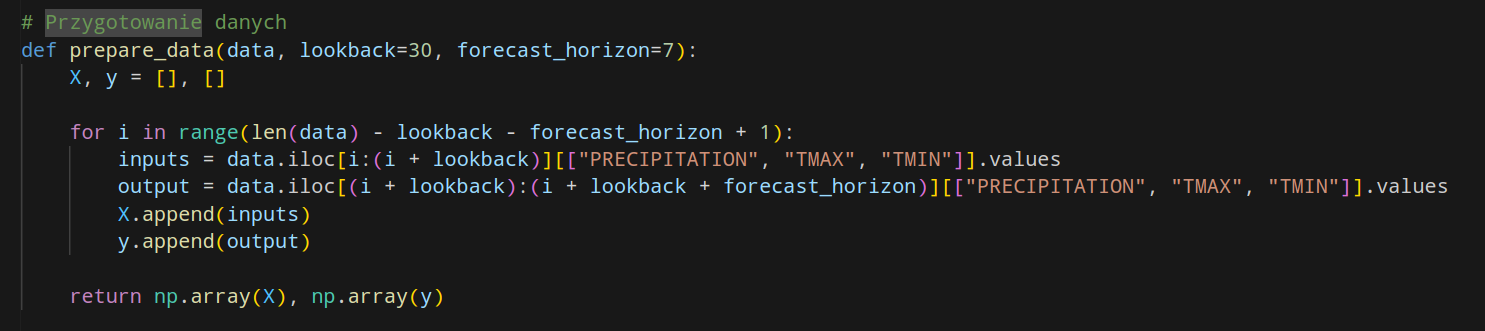
\includegraphics[width=\textwidth]{images/prepare_data.png}
        \caption{Funkcja dzieląca dane na zbiór uczący -- 30 dni i weryfikujący -- 7 dni}
    \end{figure}


    \begin{figure}
        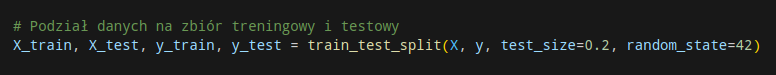
\includegraphics[width=\textwidth]{images/train_split.png}
        \caption{Funkcja z modułu sklearn \cite{split-sklearn} dzieląca na zbiór treningowy i testowy w stosunku 8:2}
    \end{figure}
\end{frame}

\begin{frame}
    \frametitle{Budowa modelu}

    \begin{figure}
        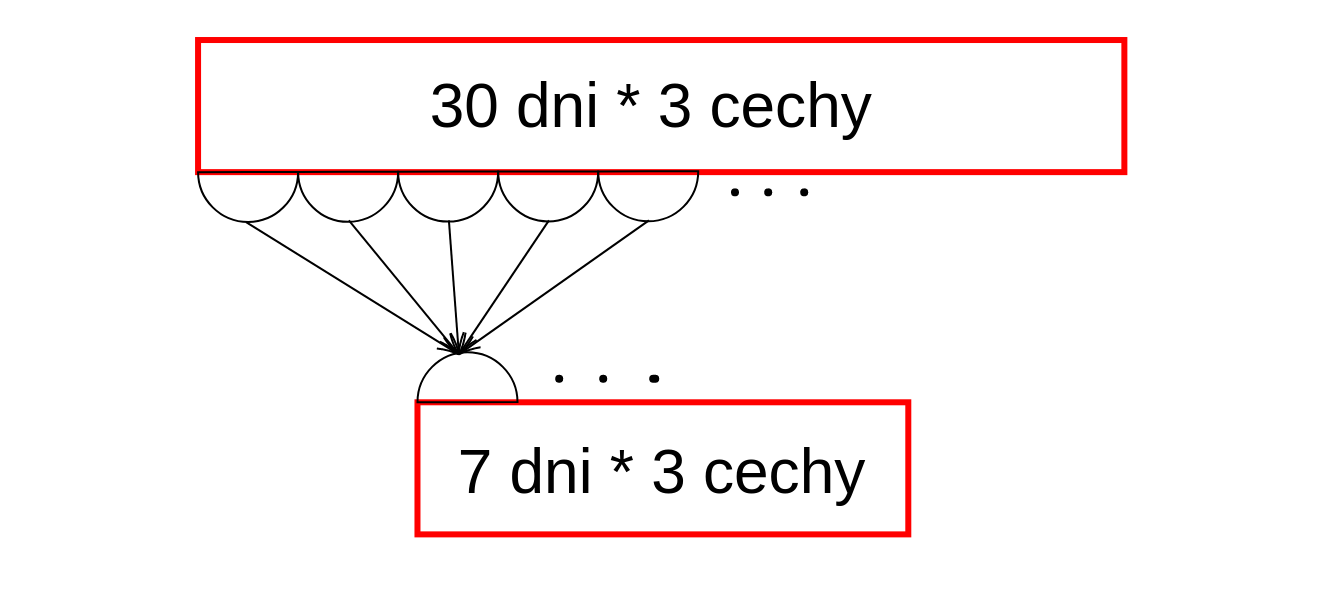
\includegraphics[width=\textwidth]{images/budowa_sieci.png}
        \caption{Model budowy sieci}
    \end{figure}

    \hspace*{1cm}

    \begin{center}
        Funkcja aktywująca "linear"
    \end{center}

\end{frame}

\begin{frame}
    \frametitle{Trenowanie modelu}

    Założenia na jakich trenowano model:
    \begin{itemize}
        \item funkcją celu było zmniejszenie błędu średniokwadratowego,
        \item wielkość serii treningowej: 16,
        \item ilość epok: 50,
        \item stosunek zbioru treningowego do testowego: 9:1.
    \end{itemize}


    \begin{figure}
        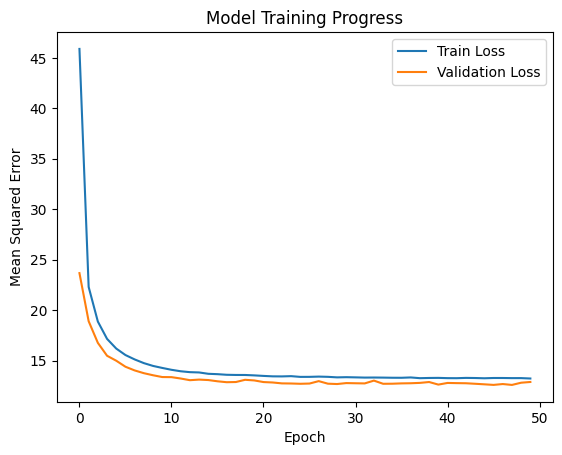
\includegraphics[width=.6\textwidth]{images/TestVsValidation.png}
        \caption{Wykres jakości modelu}
    \end{figure}

\end{frame}

\begin{frame}
    \frametitle{Wykorzystanie modelu}
    W celu przetestowania modelu przygotowano dane z serwisu pogodowego IMGW-Poland \cite{IMGW-Poland} z zakresu dni od 2023-10-01 do 2023-11-07. Stacja pogodowa Wrocław-Strachowice.

    \begin{columns}[T]
        \begin{column}{.5\textwidth}
            \begin{figure}
                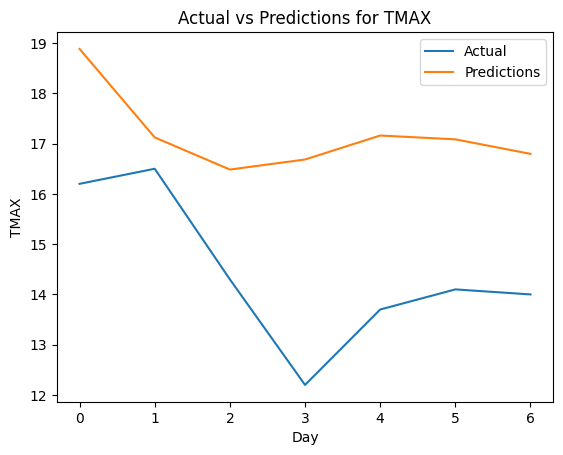
\includegraphics[width=\textwidth]{images/tmax.png}
                \caption{Wykres porównania przewidywej maksymalnej temperatury do rzeczywistych}
                \label{rys-tmax}
            \end{figure}
        \end{column}
        \begin{column}{.5\textwidth}
            \begin{figure}
                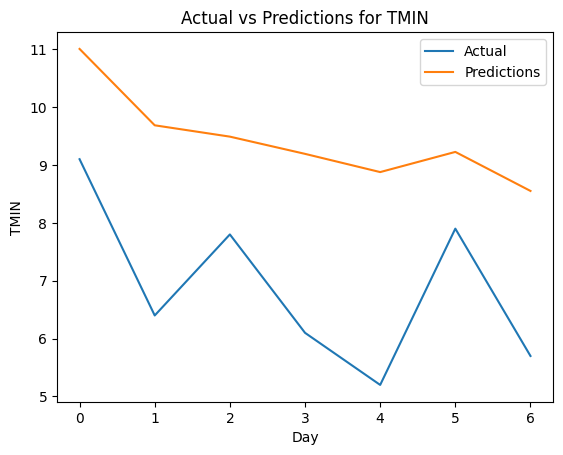
\includegraphics[width=\textwidth]{images/tmin.png}
                \caption{Wykres porównania przewidywej minimalnej temperatury do rzeczywistych}
                \label{rys-tmin}
            \end{figure}
        \end{column}
    \end{columns}

\end{frame}

\begin{frame}
    \begin{figure}
        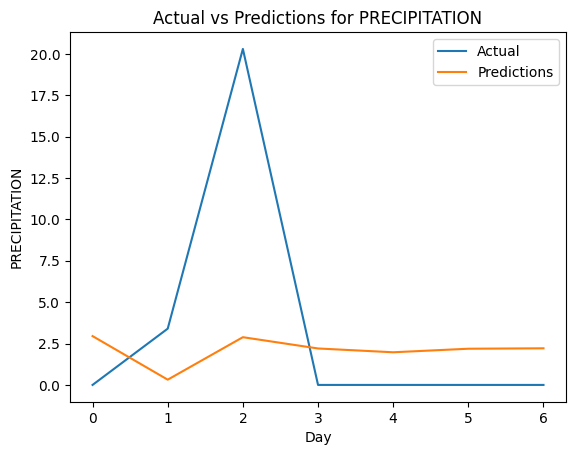
\includegraphics[width=.75\textwidth]{images/opady.png}
        \caption{Wykres porównania przewidywanych opadów do rzeczywistych}
        \label{rys-opady}
    \end{figure}
\end{frame}

\begin{frame}
    \frametitle{Podsumowanie}

    \begin{itemize}
        \item Jakość modelu oszacowana podczas treningu i walidacji wynosi $13.59$.
        \item Z rysunków \ref{rys-tmax}, \ref{rys-tmin} i \ref{rys-opady} widzimy, że wartości znacznie odbiegają od oczekiwanych wartości.
        \item Jedynie co możemy pozytywnie ocenić, to zbliżone trendy zmian wartości.
        \item W celu poprawienia jakości modelu należy rozważyć:
        \begin{enumerate}
            \item pomiary powinny pochodzić z miejsc będących w  podobnej strefie klimatycznej,
            \item uzględnić więcej danych z każdego dnia, np. średnia wartość temperatury,
            \item zastosowanie innych metod sztucznej inteligencji, np. drzewo losowe.
            \item rozważyć rozszerzenie sieci neuronowej o jeszcze jedną warstę głęboką.
        \end{enumerate}
    \end{itemize}

\end{frame}

\begin{frame}[allowframebreaks]
    \frametitle{Bibliografia}
    \bibliographystyle{ieeetr}
    \bibliography{ref.bib}

\end{frame}



\end{document}